  \documentclass{bioinfo}
  \usepackage{tipa}
  \copyrightyear{2016}
  \pubyear{2016}

  \begin{document}
  \firstpage{1}

  \title[Combined ChIP-seq discretization and quality control]{Zerone:
  a ChIP-seq discretizer for multiple replicates with built-in
  quality control}
  \author[Cusc\'o \textit{et~al}]{Pol Cusc\'o\,$^{1,2}$ and Guillaume
  Filion\,$^{1,2}$\footnote{to whom correspondence should be addressed}}
  \address{$^{1}$Genome Architecture, Gene Regulation, Stem Cells and Cancer
  Programme, Centre for Genomic Regulation (CRG), The Barcelona Institute of
  Science and Technology, Dr. Aiguader 88, Barcelona 08003, Spain.\\
  $^{2}$Universitat Pompeu Fabra (UPF), Barcelona, Spain.}
  % The CRG affiliation is compliant (October 17, 2015).

  \history{Received on XXXXX; revised on XXXXX; accepted on XXXXX}

  \editor{Associate Editor: XXXXXXX}

  \maketitle

  \begin{abstract}

  \section{Motivation:}
    Chromatin immunoprecipitation followed by high-throughput sequencing
    (ChIP-seq) is the standard method to investigate chromatin protein
    composition. As the number of community-available ChIP-seq profiles
    increases, it becomes more common to use data from different sources,
    which makes joint analysis challenging. Issues such as lack of
    reproducibility, heterogeneous quality and conflicts between
    replicates become evident when comparing data sets, especially when
    they are produced by different laboratories.

  \section{Results:}
    Here we present Zerone, a ChIP-seq discretizer with built-in quality
    control. Zerone is powered by a Hidden Markov Model with zero-inflated
    negative multinomial emissions, which allows it to merge several
    replicates into a single discretized profile. To identify low quality
    or irreproducible data, we trained a Support Vector Machine and
    integrated it as part of the discretization process. The result is
    a classifier reaching 95\% accuracy in detecting low quality profiles.
    We also introduce a graphical representation to compare discretization
    quality and we show that Zerone achieves outstanding accuracy. Finally,
    on current hardware, Zerone discretizes a ChIP-seq experiment on
    mammalian genomes in about 5 minutes using less than 700 MB of memory.

  \section{Availability:}
    Zerone is available as a command line tool and as an R package. The C
    source code and R scripts can be downloaded from
  \href{https://github.com/nanakisck/zerone}{https://github.com/nanakiksc/zerone}.
  The information to reproduce the benchmark and the figures is
  stored in a public Docker image that can be downloaded from
\href{https://hub.docker.com/r/nanakiksc/zerone/}{https://hub.docker.com/r/nanakiksc/zerone/}.

\section{Contact:}
\href{guillaume.filion@gmail.com}{guillaume.filion@gmail.com}
\end{abstract}

\section{Introduction}
One of the major challenges of biology is to understand how
transcription factors and chromatin proteins coordinate transcription,
replication and repair. In front of this colossal task, the community
invests massive research efforts into collecting protein-genome
interaction data. Chromatin immunoprecipitation followed by high
throughput sequencing (ChIP-seq) has become the standard method to
identify the targets of a transcription factor or a histone
modification in a cell population. However, ChIP is not fully
understood and artifacts are still discovered more than 10 years
after its adoption as a standard \citep{pmid24349523, pmid24173036}.
Besides, the constant improvement of sequencing technologies makes
analysis of ChIP-seq profiles difficult to standardize. There is thus
a need to continuously develop and improve computational tools to
analyse ChIP-seq data.

One of the most common analyses performed on ChIP-seq profiles is to
discretize the signal, \textit{i.e.} identify the loci where the
transcription factor (or other feature) is present.
This makes the signal simpler to interpret,
it removes part of the experimental noise, it simplifies
downstream analyses and it allows comparing or combining profiles of
different natures. This raises a challenge at the computational level
because discretization has to be carried out uniformly for signals
that may be very different. For instance, lamins bind in
megabase-scale domains covering 40\% of the genome
\citep{pmid18463634}, whereas transcription factors may bind as few
as 6~bp with a coverage below 1\%.

Large consortia such as ENCODE have brought to light
severe issues related to the quality of ChIP-seq data.
Conflicts between replicates are common, and
sometimes laboratory effects are clearly detectable in the data,
even when experimentalists use the same material and follow the same
protocol (our unpublished observations). The most popular remedy is to
use a metric called IDR \citep[Irreproducible Discovery Rate,][]{li2011},
which allows weeding
out poorly reproducible signal. This approach is a significant step
forward, but the IDR is undefined when more than two replicates are
available. Besides, keeping only the reproducible ChIP-seq peaks is not
always the best option. If one of the replicates is mislabelled,
for instance, it is more appropriate to reject the data set than to keep
the common ChIP peaks. In summary, how to integrate ChIP-seq data
from different sources and with variable qualities is still an open
problem.

Here we propose an approach to discretize ChIP-seq data where conflict
resolution and quality control are integrated in a tool that we called
Zerone\footnote{Pronounced \textipa{/zi"ro\textupsilon n/} or
\textipa{/"zi:ron/, \textit{i.e.} as inserting `ear' in `zone'}.}.
The key idea of Zerone is to combine an arbitrary number of
ChIP-seq replicates in a single discretized profile, where conflicts are
resolved by maximizing the likelihood of the underlying statistical model.
Following discretization, Zerone controls the quality of its output in
order to detect potential anomalies, and when applicable rejects the
output as a whole. Internally, the first step implements a Hidden Markov
Model (HMM) with zero-inflated negative multinomial (ZINM) emissions, and
the second implements a Support Vector Machine (SVM) trained using ENCODE
ChIP-seq data. HMM-based discretization is agnostic about
the shape of the signal (broad domains or sharp peaks) and the ZINM
distribution captures the essential features of the read count
distribution in ChIP-seq data.

Zerone is designed for large volume pipelines aiming to combine many
ChIP-seq profiles with little human intervention. To this end, it is
compatible with the standard BED, SAM/BAM, and GEM formats,
it produces congruent window-based outputs, and it can process hundreds
of experiments per day on average hardware. We benchmarked Zerone against
MACS \citep{pmid18798982}, BayesPeak \citep{pmid19772557} and
JAMM \citep{pmid25223640} on the core task of discretizing ChIP-seq
profiles of CTCF, Pol2, H3K4me3 and H3K36me3. Our results show that Zerone is
competitive in terms of speed and accuracy.

\begin{methods}
\section{Methods}

\subsection{Model and parameter estimation}
\label{sub:hmm}
It is natural to model read counts per genomic window by an unbounded
discrete distribution. The Poisson distribution is an obvious candidate,
but it is a poor choice because the variance of read counts is usually
higher than the mean for ChIP-seq data. The reason is that windows
are nonhomogeneous, which increases the dispersion. More specifically,
windows do not have the same copy numbers, they are not equally PCR-prone
and they are not equally mappable.
The negative binomial (NB) distribution is thus a better choice
because it allows some variation between windows. However, genomes
are fraught with repeats, which creates an excess of windows where
reads cannot be mapped. Since such windows will always have 0 read
count, a natural choice for this distribution is the zero-inflated
negative binomial (ZINB), \textit{i.e.} the mixture of a negative
binomial distribution and a distribution concentrated at 0
\citep{pmid21787385}.
Fig.~\ref{fig:ZINB_fit} shows that the
ZINB distribution gives a better fit to ChIP-seq data than Poisson
and NB distributions.

The ZINB distribution has 3 parameters that can be fitted by maximum
likelihood. Zerone uses a custom solver based on the Newton-Raphson
method, which converges much faster than the popular routine
\texttt{zeroinfl} \citep{psclb} from the R package
\texttt{pscl} \citep{R,pscla}.

\begin{figure}[!tpb]
\centerline{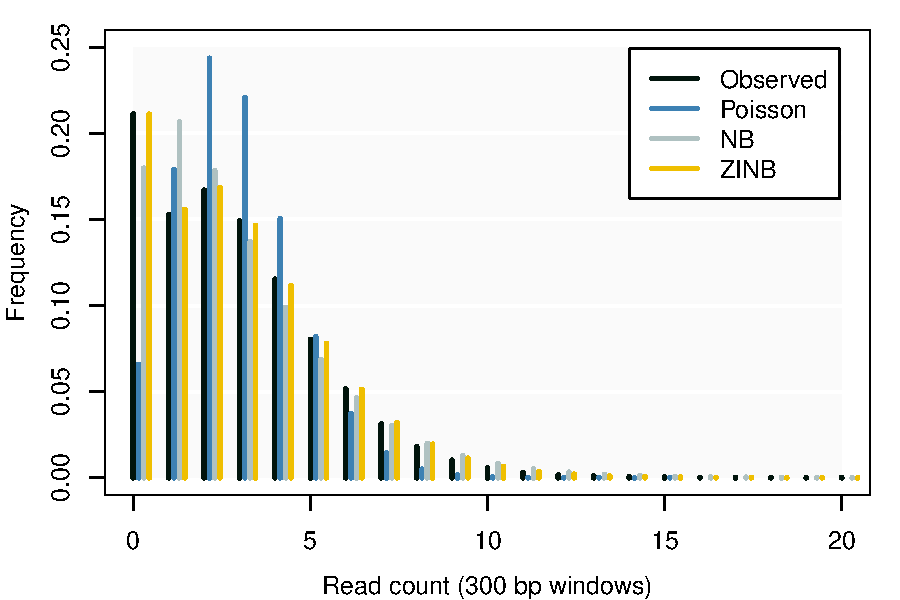
\includegraphics[scale=0.55]{ZINB_fit.pdf}}
\caption{
  Using the ZINB distribution to model ChIP-seq data (color
  version of the figure available online). Reads from
  a mock control data set were mapped onto the human genome and
  pooled in 300~bp windows after removing duplicates. The histogram of
  the read counts is shown in black (no immunoprecipitation was
  performed in this experiment, so this variation corresponds to the
  `baseline'). The colored histograms show the maximum
  likelihood fit of the Poisson, Negative Binomial (NB) and
  Zero-Inflated Negative Binomial (ZINB) distributions. The fit of
  the Poisson distribution is poor. The NB distribution
  gives a good fit at the tail, but not for windows with
  0 and 1 read. The ZINB distribution gives a good fit
  over the whole range. Source: ENCODE file ENCFF000VEK.
%\href{http://hgdownload.cse.ucsc.edu/goldenPath/hg19/encodeDCC}{http://hgdownload.cse.ucsc.edu/goldenPath/hg19/encodeDCC}.
}\label{fig:ZINB_fit}
\end{figure}

The NB distribution can be interpreted as a Gamma-Poisson process,
which gives a straightforward extension to a multivariate
distribution called the Negative Multinomial (NM) and to the
zero-inflated version of it called Zero-Inflated Negative Multinomial
distribution (ZINM, see supplementary material for detail). In this
model, windows have an intrinsic ChIP-seq bias due to their sequence
composition, mappability and other inherent properties, which gives
a baseline variation present in all ChIP-seq experiments performed
in the same cells and the same conditions. Note that the biases are
not modelled explicitly from local features of the genome (\textit{e.g.}
G+C content), but implicitly by adjusting the variance of the
distribution. Also, the ZINM distribution models the statistical
dependence between replicates and thus yields more accurate
probabilities than assuming independence.

Given that the genome contains $n$ windows, each observation
$y_i = (y_{i,1}, \ldots, y_{i,r})$ is a vector of $r$ read counts
(one per replicate), where $1 \leq i \leq n$. The associated probability
under the ZINM distribution with parameter
$\theta = (\pi, \alpha, p_0, ..., p_r)$ is

$$
g(y_i|\theta) = \left\{
\begin{array}{ll}
\pi + (1-\pi)p_0^{\alpha}
         & \mbox{if } y_i = 0 \\
(1-\pi )\frac{\Gamma(\alpha + y_{i,1} + \ldots + y_{i,r})}
  {\Gamma(\alpha)y_{i,1}! \ldots y_{i,r}!}
p_0^{\alpha} p_1^{y_{i,1}} \ldots p_r^{y_{i,r}}
         & \mbox{otherwise.}
\end{array}
\right.
$$

In the definition above, $\Gamma$ denotes Euler's gamma function and
$y_i = 0$ stands for the multiple equality $y_{i,1} = \ldots = y_{i,r} = 0$.
$\pi$ is the zero-inflation or mixture parameter (the proportion of
unmappable windows), $\alpha$ is a shape parameter dictating the
distribution of reads and $p_0, \ldots, p_r$ are probabilities linked
by the equality $p_0 + p_1 + \ldots + p_r = 1$ and dictating the average
number of reads per window for each replicate.

Discretization is performed by fitting an HMM
with ZINM emissions. The HMM has three
states corresponding to ``low'', ``medium'' and ``high'' abundance of
the given chromatin feature. In many ChIP-seq
profiles, the baseline signal shows piece-wise variations of low amplitude
but large size (typically 10-100 Kb). This will sometimes be the dominant
signal and a two-state HMM will identify these blocks instead of the
targets. Dedicating two states to fit the baseline is a way to make sure
that the ``high'' state corresponds to the targets of the chromatin
feature. In what follows, targets always correspond to
the ``high'' state.

Assuming that $x_i$ takes one of these three values, the log-likelihood of
a sequence of states $(x_1, \ldots, x_n)$ given the observations
$(y_1, \ldots, y_n)$ is

$$
\log \nu(x_0) + \log g(y_0|x_0) +
   \sum_{i=1}^n \log Q(x_{i-1},x_i) + \log g(y_i|x_i).
$$

In the above, $\nu$ denotes the initial probabilities of the states,
$Q$ is the $3 \times 3$ transition matrix of the model, and
$g(y_i|x_i)$ is the probability of the emission $y_i$ if the state is
$x_i$ (the parameter vector $\theta$ depends on the state of the HMM).
Discretization amounts to finding the sequence of states and the
model parameters that maximize the value above. Zerone achieves this
with the Baum-Welch algorithm \citep{baum1966}, which is a special case
of the EM algorithm \citep{Dempster77maximumlikelihood}. The emission
parameters $\pi$ and $\alpha$ are state-independent since they represent
the baseline distribution of reads in the genomic windows. For this
reason they are fitted from the negative control profiles before the
Baum-Welch cycles (as a side note, fitting them with the Baum-Welch
algorithm sometimes lead to aberrant solutions). The other parameters
are state-dependent since they represent the amount of reads per window
in each replicate, depending on the abundance of the chromatin feature.
Overall, the total number of estimated parameters is $3r+9$, where $r$
is the number of replicate experiments.

The fitting process resolves conflicts between replicates. Say that
a ChIP-seq peak is present in only one of them; the signal
will be locally high only for this replicate and low for the others.
Because of the conflict, the local log-likelihood will be low for
all the possible states but there will still be an optimum that
corresponds to the `least unlikely' state. The final call depends on
whether the weight of evidence is higher for the presence of the
peak or for its absence. If the conflict is strong, the confidence
in the final call will be weak, which can lead to a rejection of
the profile as a whole if such cases are too frequent (see below).

Transition parameters are updated through the forward-backward
algorithm \citep{18626}, and emission parameters are updated by solving
maximum likelihood equations with the Newton-Raphson method (see
supplementary material for detail). The state calls are computed by
finding the most likely segmentation given the value of the parameters
through the Viterbi algorithm \citep{1054010}.

\subsection{ChIP-seq preprocessing}
Mapped reads are binned in fixed-step windows (default 300
bp) by their mid-point and PCR duplicates (\textit{i.e.} reads mapping to
the same location in the same orientation) are removed. The window size
should not be smaller than the sonication fragment length and
it should be set so that there are on average more than 3-4 mapped reads
per window. Zerone decompresses gzipped input files if required. There is
no upper limit to the number of input files to discretize simultaneously,
but there must be at least one negative control and one ChIP-seq experiment.

\subsection{Quality control}
\label{sub:training}
We used a machine learning strategy to identify discretization
failures. The true status (success or failure) of experimental ChIP-seq
data is not known because success is partly subjective and because
there is no gold standard for protein binding in live cells.
We prepared an experimental data set where we labelled the
output of Zerone as positive (success) or negative (failure) based
on empirical criteria (see associated Docker container for detail).
The definition of success is thus subjective, but the training is
performed on representative data.

We discretized 96 replicated ChIP-seq experiments together with their
respective input control (see associated Docker container). Based on
visual inspection and on the available literature, we determined
that discretization was successful in 91 cases that consituted the
positive examples of our training set. The most common cases of
poor data quality in ChIP-seq correspond to low signal-to-noise ratio
(\textit{e.g.} when the antibody is not specific), and lack of
reproducibility between replicates (\textit{e.g.} when samples are
swapped). We created 91 negative cases obtained by discretizing
nonreplicate profiles (\textit{e.g.} CTCF and Pol2) or controls without
immunoprecipitation. Thus, a total of 182 cases (91 positive and 91
negative) were used to build a balanced data set. We extracted 5
features from the output of Zerone to train a classifier:
the transition matrix entry $Q_{2,0}$ (indicating the size of the
targets), the minimum value of the ratios
$p_2(2)/p_2(1), \ldots, p_r(2)/p_r(1)$ (indicating the
signal to noise ratio), the amount of targets, the fraction of
variance explained by the discretization and the correlation between
replicates.


\begin{figure}[!tpb]
\centerline{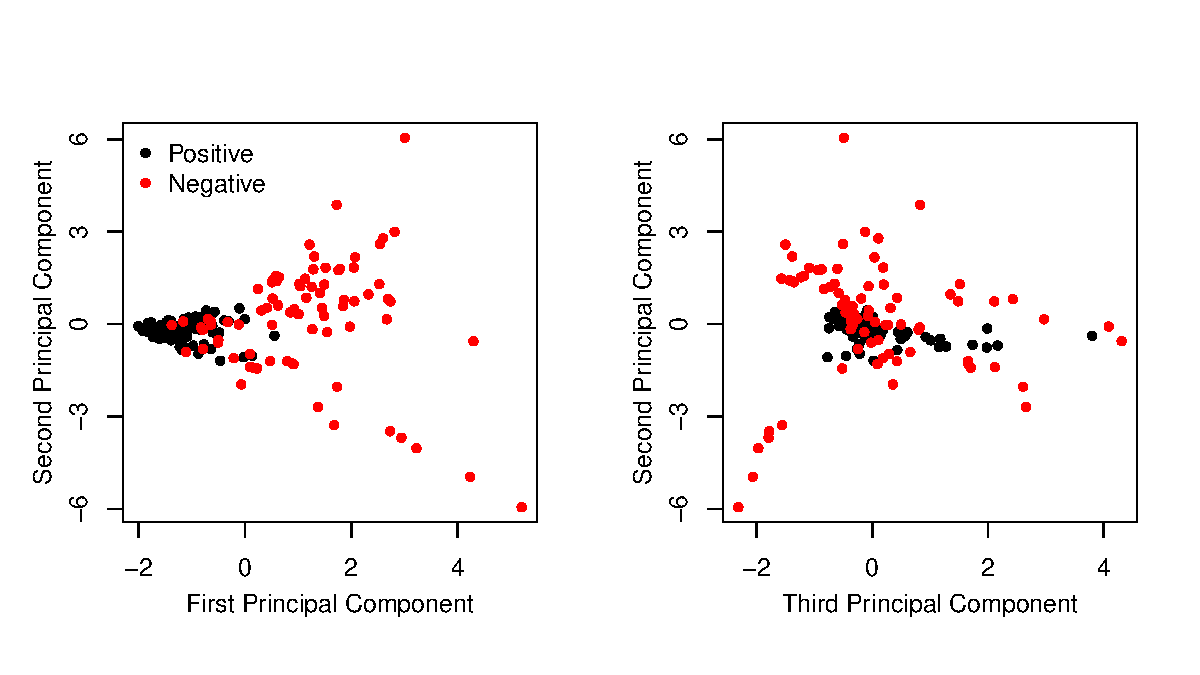
\includegraphics[scale=0.45]{PCA.pdf}}
\caption{
  Scaled Principal Component Analysis of the training data set
  (color version of the figure available online).
  Each symbol represents a discretization performed by Zerone. The
  5 features extracted from each discretization are projected onto
  the first three principal components. The two groups overlap,
  which creates an ambiguous zone where failures and successes are
  indistinguishable.
}\label{fig:pca}
\end{figure}


To separate the points in the feature space (Fig.~\ref{fig:pca}),
we used a Support Vector Machine (SVM, \citealp{Chang2011,e1071}),
as SVMs allow non linear classification, are fast to train and
require only one hyperparameter to be fitted.
We trained the SVM with a radial basis function kernel and
selected the hyperparameters that maximized the prediction
performance on test sets using a 10-fold cross-validation scheme.
The prediction accuracy on the training set was 95\%. Unlike
quality control methods based on individual peaks (such as the
IDR for instance) the quality control implemented in Zerone is
`all-or-none', \textit{i.e.} the profile is rejected or accepted
as a whole.

\subsection{Benchmark data sets and conditions}
\label{sub:bench_cond}
We used all the ChIP-seq fastq files produced by the ENCODE Consortium
on the human leukemia cell line K562. Reference assembly UCSC hg19 was
used throughout. The data was downloaded from the repository
\href{http://hgdownload.cse.ucsc.edu/goldenPath/hg19/encodeDCC}{http://hgdownload.cse.ucsc.edu/goldenPath/hg19/encodeDCC} in November 2013.
We mapped all the raw reads on the human genome with
GEM \citep[gem-mapper version 1.376 beta, gem-indexer version
1.423 beta,][]{pmid23103880}, using the options \texttt{--unique-mapping} and
\texttt{-q ignore}. We converted the mapped files to SAM format with
gem-2-sam version 1.423 beta.

To compare Zerone to other discretizers, we analysed four different
ChIP-seq data sets: CCCTC-binding factor (CTCF), RNA polymerase II
(Pol2), tri-methylated histone H3 at lysine 4 (H3K4me3)
and tri-methylated histone H3 at lysine 36 (H3K36me3).
Each data set consists of a mock profile without immunoprecipitation
and two replicate ChIP-seq profiles.
The ENCODE accession numbers for these four data sets are
ENCSR000DWE, ENCSR000FAJ, ENCSR000DWB and ENCSR000DWD respectively.
For the Pol2 data set, we used the control experiment ENCSR000EWK.
Table~\ref{tab:summary} gives a global overview of the data sets.

\begin{table}[!tbp]
\processtable{Summary statistics of the data sets used for benchmarking.
\label{tab:summary}}
{\begin{tabular}{lrrr}
        \toprule
        \textbf{Data set} & \textbf{Read size} &
        \textbf{Sequencing depth} & \textbf{Mapped reads} \\
        \midrule
        Input            & 36 & 18,123,856 & 18,064,246 \\
        Input (Pol2)     & 36 & 36,418,708 & 36,351,513 \\
        CTCF$^{(1)}$     & 36 & 32,740,518 & 15,698,068 \\
        CTCF$^{(2)}$     & 36 & 27,953,212 & 12,971,023 \\
        Pol2$^{(1)}$     & 36 & 10,513,992 &  7,465,806 \\
        Pol2$^{(2)}$     & 36 & 10,855,446 &  7,027,761 \\
        H3K4me3$^{(1)}$  & 36 & 18,685,398 & 15,148,578 \\
        H3K4me3$^{(2)}$  & 36 & 16,968,870 & 13,656,987 \\
        H3K36me3$^{(1)}$ & 36 & 18,174,968 & 13,847,015 \\
        H3K36me3$^{(2)}$ & 36 & 18,495,290 & 14,419,200 \\
        \botrule
\end{tabular}}{The input profile marked as Pol2 was used to discretize the
Pol2 profiles. All the other profiles were discretized with the other input.
The numbers in parentheses indicate the two experimental replicates.}
\end{table}

We tested MACS \texttt{callpeak} version 2.1.0.20140616, BayesPeak
version 1.20.0 and JAMM version 1.0.7rev1. All tests were performed on
an 8-core Intel Xeon E5606 machine with 48~GB of DDR3-RAM at 1333~MHz.
All programs were run on a single core with the recommended options.
Specifically, on the H3K36me3 data set, JAMM was run with the option
\texttt{-r region} and MACS with the \texttt{--broad} option. For the rest of
the data sets and programs, the default options were used.
When using IDR, we ran MACS with a relaxed qvalue cutoff set to 0.05
to obtain a higher number of peaks. The IDR analysis proper was conducted
using the R script \texttt{batch-consistency-analysis.r}, available at
\href{https://sites.google.com/site/anshulkundaje/projects/idr}{https://sites.google.com/site/anshulkundaje/projects/idr}.
Peaks scoring higher than 0.05 were ignored.

The CTCF motif was obtained from the JASPAR database version
5.0{\textunderscore}ALPHA \citep[motif ID MA0139.1,][]{pmid24194598}.
Subsequently we used FIMO \citep{pmid21330290} from the MEME suite version
4.10.1 \citep{pmid19458158} to identify and map CTCF motif occurences in
the human genome. The positions of TSS were extracted from the knownGene
table of the UCSC Genes annotation \citep{Karolchik2004}.
Gene expression in sections \ref{subsub:pol2} and \ref{subsub:h3k4me3}
was determined from a genomic run-on sequencing (GRO-seq)
data set on the cell line K562 (GEO accession GSM1480325).
All the genomic features overlapping with at least one GRO-seq tag
were considered to be expressed.
RNA counts in section \ref{subsub:h3k36me3} were obtained from the
ENCODE data set EH000163 (already mapped .bigWig files).

The quality control of Zerone was compared to the IDR-based method
for flagging replicates with low consistency. Briefly, pairwise
comparisons are performed between all the replicates to check that
the number of reproducible peaks is similar between them. The
same comparisons are also performed between random splits of each
replicate, and between random splits of a pooled profile. Experiments
that do not satisfy these conditions are flagged as faulty (see
associated Docker container for detail).

A full replay of the benchmark including all the necessary data sets
is available from the associated Docker image.

\end{methods}

\section{Results}
\label{sec:results}

\subsection{Automatic quality control}

\begin{figure}[!tpb]
\centerline{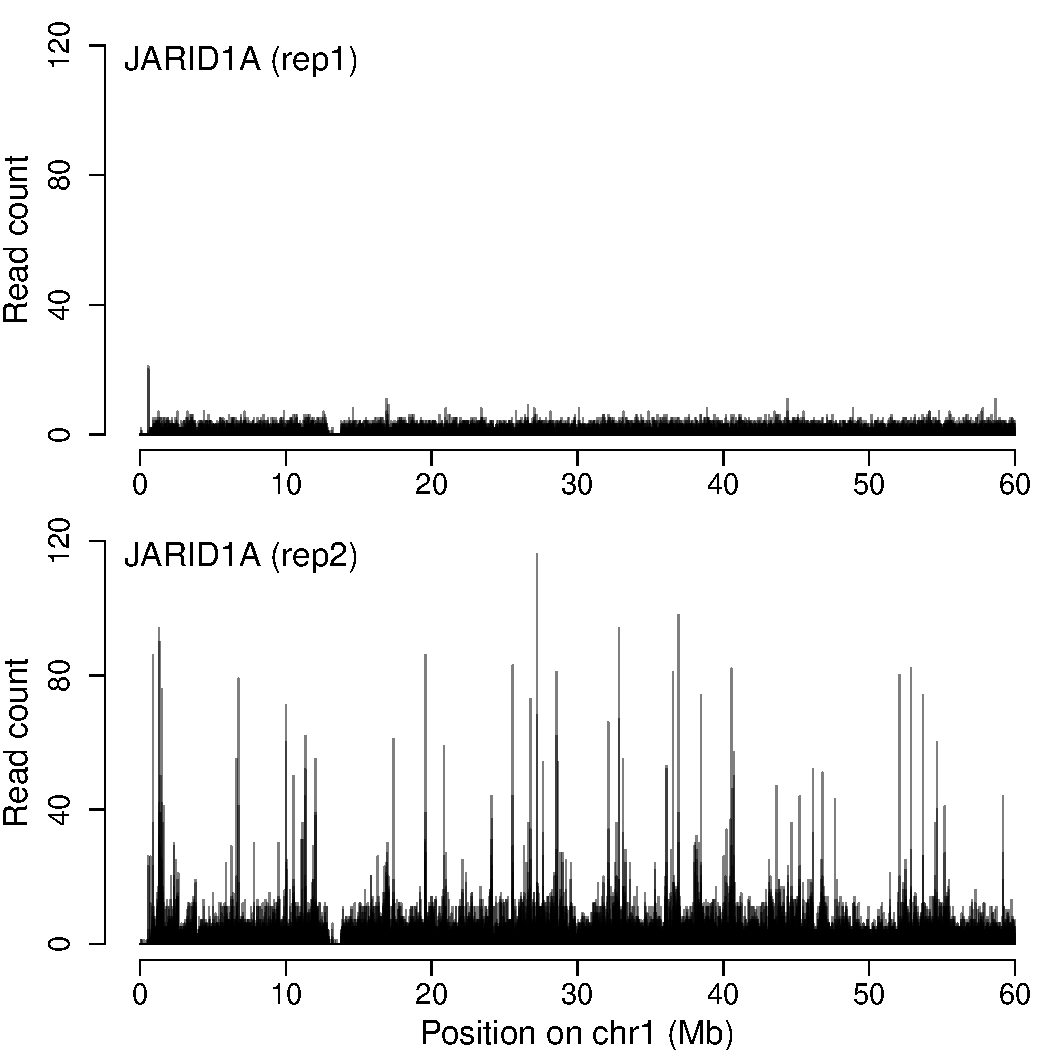
\includegraphics[scale=0.5]{jarid.pdf}}
\caption{
  ChIP-seq profiles of JARID1A in H1 ES cells (300 bp windows).
  The first replicate is not similar to the second, and it does not
  contain any target.
}\label{fig:jarid}
\end{figure}

The most novel feature of Zerone is an embedded automatic quality
control step taking place after the discretization. It not only
ensures that the discretization is sensible, but also that the
replicates are similar to each other and that the ChIP-seq profiles
are not too similar to the mock controls. Our approach is based
on the idea that discretizations from overly noisy or
divergent profiles should have a signature that
can be picked up by a specially trained classifier.

We identified 5 summary statistics that characterize the quality of
the discretization and trained an SVM to recognize failures. We thus
obtained a classifier able to identify a failed discretization with
95\% accuracy (see section \ref{sub:training}).

This feature is essential for high throughput automatic pipelines.
For instance, when discretizing ENCODE ChIP-seq profiles obtained in
human H1 ES cells, we noticed that the lysine-demethylase JARID1A did
not pass the quality control.
Further investigation immediately revealed the nature of the issue.
In one of the replicates, the signal is lacking entirely, as if
the immunoprecipitation failed (Fig.~\ref{fig:jarid}).
Once aware of the issue, users can handle it properly (for instance,
by discarding the protein or by working with a single replicate).
Without automatic quality control, the low quality of the first replicate
would have been missed.

Low quality profiles can also be detected using IDR. On a test
set of 30 chromatin features from H1 ES cells, we obtained 85\%
agreement between the quality control of Zerone and discretization
with MACS followed by IDR-based flagging (see section
\ref{sub:bench_cond} and associated Docker
container). It is important to note that IDR does not apply to
profiles with broad domains and that it represents a significant
computational burden when there are many replicates or many targets
sites.

\subsection{Accuracy}

\begin{figure}[!tpb]
\centerline{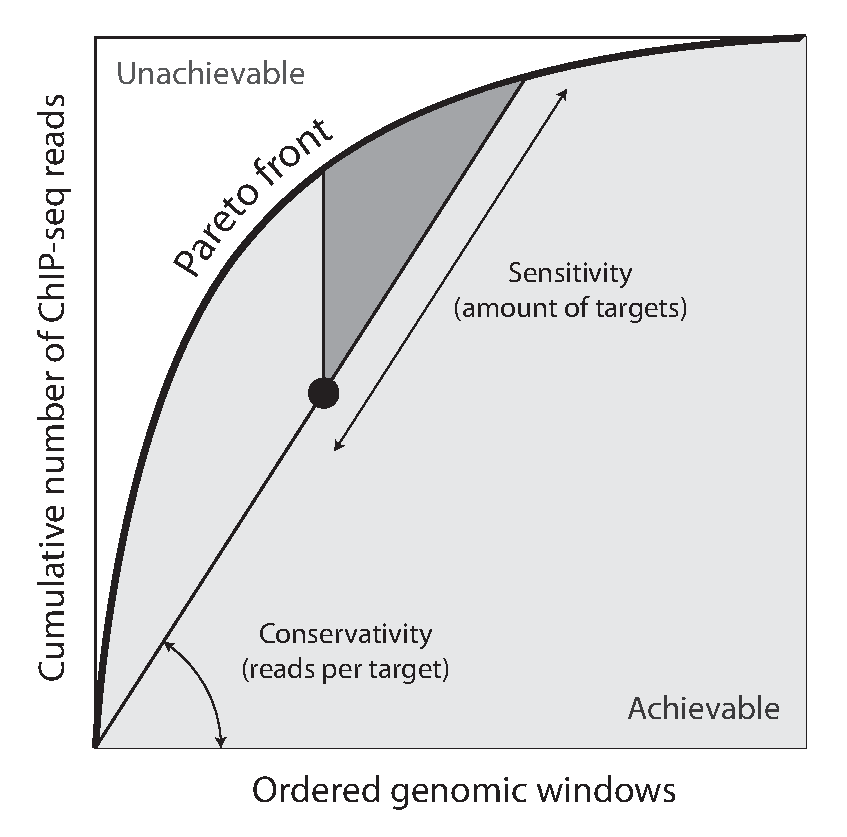
\includegraphics[scale=0.5]{pareto_front_explanation.pdf}}
\caption{
  Graphical representation of discretizations. Genomic
  windows of the ChIP-seq profile are ordered by decreasing amount of
  reads on the $x$ axis, and the cumulative amount of reads is plotted
  on the $y$ axis. This line forms a Pareto front representing the
  maximum number of reads for a given number of windows. Discretizations
  are represented as a single point on this plane (black disc) whose
  coordinates are the number of targets and the total number of reads
  covered by the targets. The dark triangle represents discretizations
  that are more conservative and discover more targets.
}
\label{fig:expl}
\end{figure}

\begin{figure*}[!tbp]
\centerline{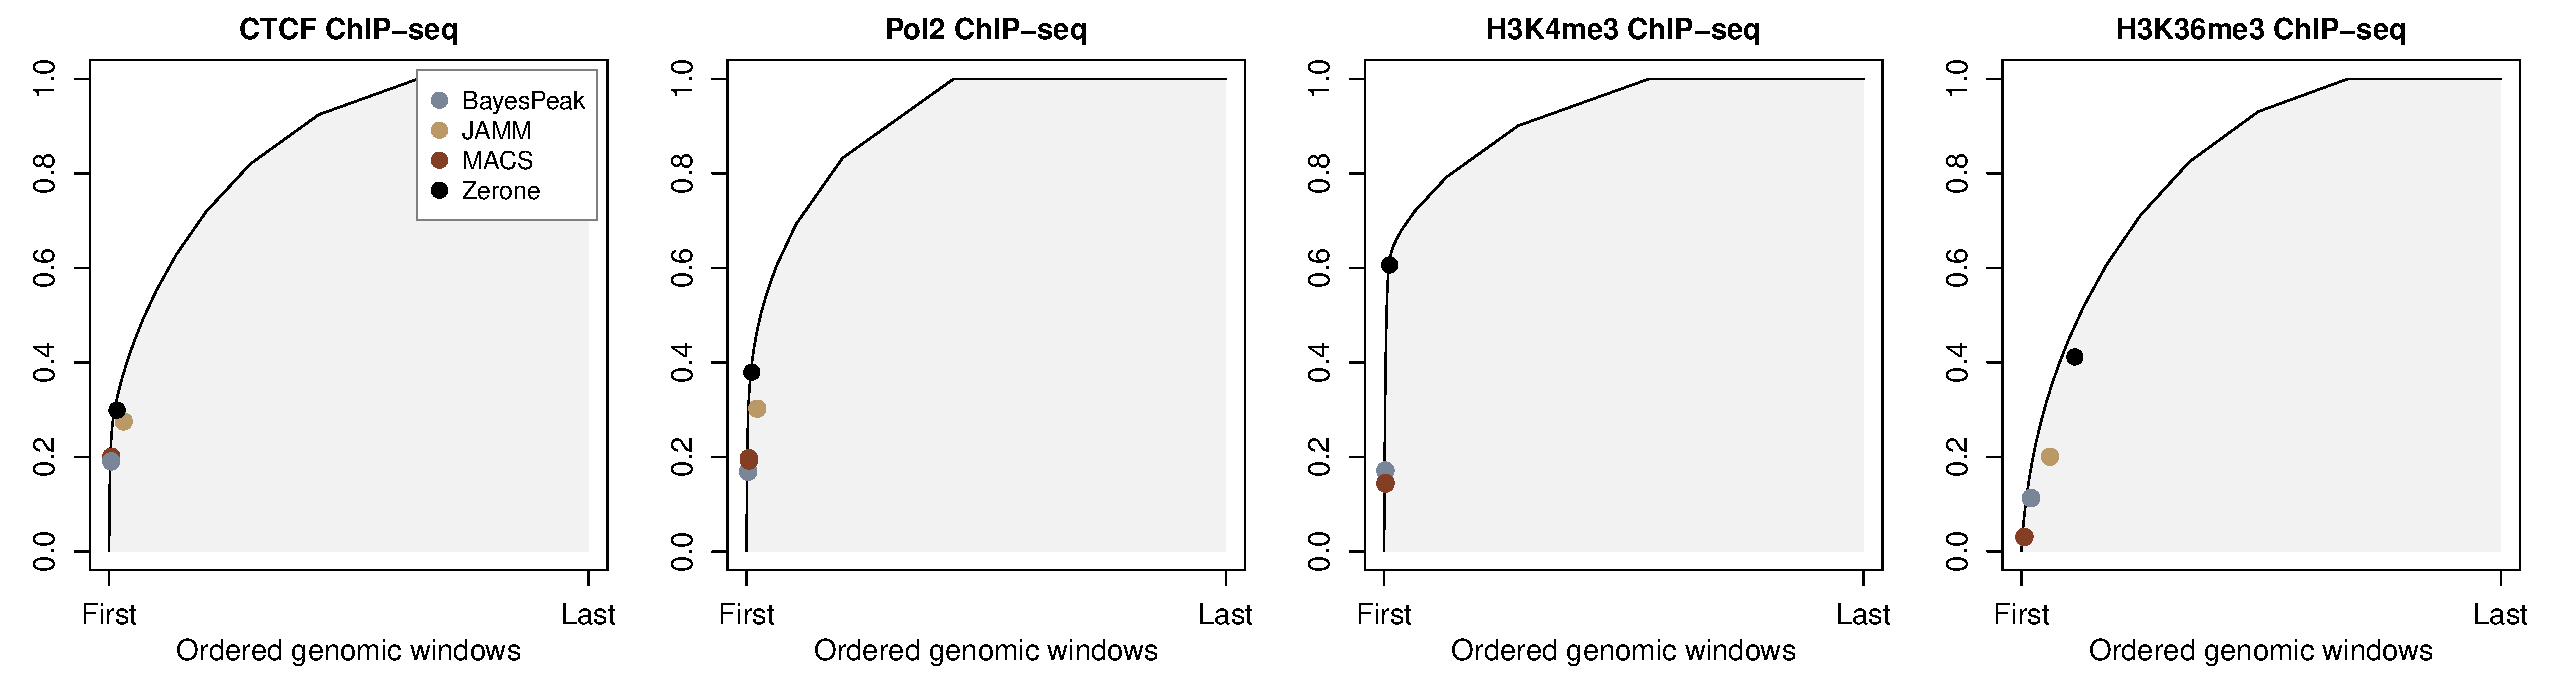
\includegraphics[scale=0.4]{pareto_front.pdf}}
\caption{
  Characteristics of the discretizations for different programs
  (color version of the figure available online).
  The representation is obtained as shown on Fig.~\ref{fig:expl}.
  When discretizing the CTCF, the Pol2 and the H3K4me3 profile,
  Zerone produces discretizations that are very close to the Pareto
  front. In the case of H3K36me3, the discretization is off the
  Pareto front, but it is more sensible than the others.
}
\label{fig:pareto}
\end{figure*}

The purpose of discretizers is to identify the targets of a
transcription factor or a histone mark, \textit{i.e.} the sites of
the genome where it is present.
Intuitively, good discretizers capture a large fraction of the
ChIP-seq signal within few targets. The number of targets
and the amount of reads they represent are therefore critical
characteristics of a discretization. Unfortunately, there is no gold
standard to estimate the trade-off between false positives and false
negatives in ChIP-seq experiments, and thus there is no objective way
to rank discretizers \citep{pmid21059603}. However, we can compare
them with a partial order, as explained below.

When arranging genomic windows from high to low amount of ChIP-seq
reads, the cumulative number of reads forms a Pareto front.
It represents the largest amount of reads that can be captured by the
given amount of targets (Fig.~\ref{fig:expl}). A discretization can
be represented as a point on the $xy$ plane.  By construction, no
discretization can lie on the left of the Pareto front, and those on
the front represent an optimum. Others are suboptimal, since it is
possible to capture more reads with the same amount of targets.

We benchmarked Zerone against three ChIP-seq discretizers.
We included MACS as the standard method for ChIP-seq peak calling,
BayesPeak because it is powered by an HMM with ZINB emissions
similar to the model implemented in Zerone, and JAMM because, as
Zerone, it can perform joint discretization of experimental replicates.

This representation reveals that discretizing the CTCF profile yields
similar outputs regardless of the software (Fig.~\ref{fig:pareto},
left panel). On the other hand, discretizing the Pol2, the H3K4me3 or
the H3K36me3 profile yields very distinct outputs. In
all the cases, Zerone produces the discretization capturing the most
reads. For CTCF, Pol2 and H3K4me3 it lies on the Pareto front. For
H3K36me3, it lies somewhat off the Pareto front, but at a sensible
location. As detailed below, H3K36me3 is deposited on transcribed
genes \citep{pmid16122420,pmid23739122} so the coverage is expected to
be higher than for transcription factors. Taken together, this data
shows that Zerone produces discretizations that are sensitive and
adapted to the profile being discretized.

\subsubsection{Identification of CTCF binding sites.}
CTCF binds a 20~bp consensus sequence that is highly conserved in
vertebrates. In humans, nearly 80\% of the CTCF binding sites contain
the consensus motif \citep{pmid17382889}. In order to determine the
capacity of the different programs to call peaks of CTCF binding, we
compared the discretized profiles against a data set of CTCF binding
motifs. We obtained a reference data set containing the positions of
85,690 occurences of the CTCF motif (see section
\ref{sub:bench_cond}).

Table~\ref{tab:ctcf} shows that Zerone has the best $F_1$ score (the
harmonic mean of precision and recall) and the second highest recall
score, close to that of JAMM. On the other hand, several other tools
have a higher precision, especially when used with IDR.

\begin{table}[!b]
\processtable{Performance on the CTCF motifs data set.
True and false positives are defined as peaks with and without a CTCF
motif, respectively. Total: number of peaks found by the program.
Motif: subset of those containing at least one CTCF motif.
Precision: Motif divided by Total. Recall: number of motifs covered
by peaks divided by the number of motifs in the genome. $F_{1}$ score:
harmonic mean between Precision and Recall.
\label{tab:ctcf}}
{\begin{tabular}{lrrccc}
        \toprule
        \textbf{Software}  & \textbf{Total}  & \textbf{Motif} &
        \textbf{Precision} & \textbf{Recall} & \textbf{$F_{1}$ score} \\
        \midrule
        BayesPeak$^{(1)}$  &  45,229 & 24,933 & 0.55 & 0.31 & 0.40 \\
        BayesPeak$^{(2)}$  &  45,192 & 23,136 & 0.51 & 0.29 & 0.37 \\
        JAMM               & 321,263 & 31,859 & 0.10 & 0.39 & 0.16 \\
        JAMM$^{(1)}$ + IDR &   7,201 &  5,159 & 0.72 & 0.07 & 0.12 \\
        JAMM$^{(2)}$ + IDR &   7,201 &  5,159 & 0.72 & 0.07 & 0.12 \\
        MACS$^{(1)}$       &  48,341 & 26,129 & 0.54 & 0.32 & 0.41 \\
        MACS$^{(2)}$       &  41,048 & 23,237 & 0.57 & 0.29 & 0.38 \\
        MACS$^{(1)}$ + IDR &  25,080 & 17,488 & 0.70 & 0.22 & 0.33 \\
        MACS$^{(2)}$ + IDR &  25,080 & 17,483 & 0.70 & 0.22 & 0.33 \\
        Zerone             &  54,315 & 28,738 & 0.53 & 0.38 & 0.44 \\
        \botrule
\end{tabular}}{The numbers in parentheses indicate the results on the two
replicates separately.}
\end{table}

In summary, Zerone achieves a good balance between sensitivity and
specificity for transcription factor profiles, as was suggested by
the left panel of Fig.~\ref{fig:pareto}.

\subsubsection{Pol2 binding around transcription start sites.}
\label{subsub:pol2}
To compare the behavior of the discretizers on the Pol2 profile,
we determined the extent to which the enriched regions contained
Transcription Start Sites (TSS), as Pol2 is expected to bind near
annotated TSS. We also overlapped this annotation with a data set of
gene expression obtained by GRO-seq in order to separate the
promoters of transcribed from nontranscribed genes.

\begin{table*}[!tbp]
\processtable{Performance on the Pol2 data set.
True and false positives are defined as peaks with and without a
transcription start site (TSS), respectively. Total: number of peaks
found by the program. TSS: subset of those containing at least one
TSS. Precision: TSS divided by Total. Recall: number of TSS covered
by peaks divided by the number of TSS in the genome. $F_{1}$ score:
harmonic mean between Precision and Recall.
\label{tab:tss}}
{\begin{tabular}{lr|rccc|rccc}
        \multicolumn{2}{c}{} & \multicolumn{4}{c}{\textbf{All TSS}} & \multicolumn{4}{c}{\textbf{Active TSS}} \\
        \midrule
        \textbf{Software} & \textbf{Total} &
        \textbf{TSS} & \textbf{Precision} & \textbf{Recall} & \textbf{$F_{1}$ score} &
        \textbf{TSS} & \textbf{Precision} & \textbf{Recall} & \textbf{$F_{1}$ score} \\
        \midrule
        BayesPeak$^{(1)}$  &  32,758 & 5,877 & 0.18 & 0.15 & 0.16 & 5,127 & 0.16 & 0.34 & 0.21 \\
        BayesPeak$^{(2)}$  &  35,310 & 5,783 & 0.16 & 0.15 & 0.15 & 5,055 & 0.14 & 0.33 & 0.20 \\
        JAMM               & 239,637 & 5,514 & 0.02 & 0.13 & 0.04 & 4,728 & 0.02 & 0.29 & 0.04 \\
        JAMM$^{(1)}$ + IDR &  18,152 & 4,141 & 0.23 & 0.10 & 0.14 & 3,774 & 0.21 & 0.24 & 0.22 \\
        JAMM$^{(2)}$ + IDR &  18,152 & 4,100 & 0.23 & 0.10 & 0.14 & 3,761 & 0.21 & 0.24 & 0.22 \\
        MACS$^{(1)}$       &  51,271 & 6,860 & 0.13 & 0.17 & 0.15 & 5,920 & 0.12 & 0.39 & 0.18 \\
        MACS$^{(2)}$       &  49,062 & 6,552 & 0.13 & 0.16 & 0.15 & 5,704 & 0.12 & 0.37 & 0.18 \\
        MACS$^{(1)}$ + IDR &  19,369 & 5,985 & 0.31 & 0.15 & 0.21 & 5,307 & 0.27 & 0.36 & 0.31 \\
        MACS$^{(2)}$ + IDR &  19,369 & 5,875 & 0.30 & 0.15 & 0.20 & 5,239 & 0.27 & 0.35 & 0.31 \\
        Zerone             &  25,703 & 7,673 & 0.30 & 0.21 & 0.25 & 6,547 & 0.25 & 0.47 & 0.33 \\
        \botrule
\end{tabular}}{The numbers in parentheses indicate the results on the two
replicates separately.}
\end{table*}

Table~\ref{tab:tss} shows that Zerone obtains the highest $F_1$
score. Here the precision of Zerone is almost as high at that of MACS
+ IDR, with a better recall. These results confirm that the performance
of Zerone is good on this data set, as suggested by the middle panel of
Fig.~\ref{fig:pareto}.

\subsubsection{H3K4me3 signal on active promoters.}
\label{subsub:h3k4me3}
The histone mark H3K4me3 is enriched on active promoters and
near the TSS of actively transcribed genes
\citep{pmid15680324,pmid17512414,pmid17277777}. It is thus an example
of histone mark forming narrow peaks. We used the same TSS data set
as above to benchmark the accurary of Zerone when discretizing
this profile.

\begin{table*}[!t]
\processtable{Performance on the H3K4me3 data set.
True and false positives are defined as peaks with and without a
transcription start site (TSS), respectively. Total: the number of peaks
found by the program. TSS: the subset of those containing at least one
TSS. Precision: TSS divided by Total. Recall: the number of TSS contained
in the peaks divided by the number of TSS in the genome. $F_{1}$ score: the
harmonic mean between Precision and Recall.
\label{tab:H3K4}}
{\begin{tabular}{lr|rccc|rccc}
        \multicolumn{2}{c}{} & \multicolumn{4}{c}{\textbf{All TSS}} & \multicolumn{4}{c}{\textbf{Active TSS}} \\
        \midrule
        \textbf{Software} & \textbf{Total} &
        \textbf{TSS} & \textbf{Precision} & \textbf{Recall} & \textbf{$F_{1}$ score} &
        \textbf{TSS} & \textbf{Precision} & \textbf{Recall} & \textbf{$F_{1}$ score} \\
        \midrule
        BayesPeak$^{(1)}$  &  26,938 & 4,330 & 0.16 & 0.12 & 0.13 & 3,507 & 0.13 & 0.25 & 0.17 \\
        BayesPeak$^{(2)}$  &  27,132 & 4,288 & 0.16 & 0.11 & 0.13 & 3,468 & 0.13 & 0.24 & 0.17 \\
        JAMM               & 151,655 & 3,644 & 0.02 & 0.09 & 0.04 & 2,665 & 0.02 & 0.18 & 0.03 \\
        JAMM$^{(1)}$ + IDR &  24,065 & 3,610 & 0.15 & 0.10 & 0.12 & 2,901 & 0.12 & 0.20 & 0.15 \\
        JAMM$^{(2)}$ + IDR &  24,065 & 3,773 & 0.16 & 0.10 & 0.12 & 3,028 & 0.13 & 0.21 & 0.16 \\
        MACS$^{(1)}$       &  29,125 & 6,614 & 0.23 & 0.18 & 0.20 & 5,222 & 0.18 & 0.38 & 0.24 \\
        MACS$^{(2)}$       &  29,420 & 6,542 & 0.22 & 0.18 & 0.20 & 5,183 & 0.18 & 0.37 & 0.24 \\
        MACS$^{(1)}$ + IDR &  20,037 & 6,384 & 0.32 & 0.18 & 0.23 & 5,087 & 0.25 & 0.37 & 0.30 \\
        MACS$^{(2)}$ + IDR &  20,037 & 6,348 & 0.32 & 0.18 & 0.23 & 5,068 & 0.25 & 0.37 & 0.30 \\
        Zerone             &  15,602 & 6,989 & 0.45 & 0.20 & 0.28 & 5,528 & 0.35 & 0.41 & 0.38 \\
        \botrule
\end{tabular}}{The numbers in parentheses indicate the results on the two
replicates separately.}
\end{table*}

Table~\ref{tab:H3K4} shows that Zerone achieves better $F_1$ score,
better precision and better recall than the other tools, with
a neat advantage in precision. In this case, discarding the
nonreproducible peaks found by MACS only gives a mild increase in
precision, that does not reach the performance of Zerone.
This shows that Zerone accurately describes profiles of this category.

\subsubsection{H3K36me3-enriched domains on active genes.}
\label{subsub:h3k36me3}
There is no consensus sequence to determine the location of histone
modifications. However, it is known that the bodies of active genes
are enriched in H3K36me3 \citep{pmid16122420,pmid23739122}. Therefore,
the genes that contain peaks or windows determined as enriched in
H3K36me3 by the different discretizers should be more expressed than
the background.

We benchmarked the quality of the discretization with expression
data obtained in the same cell. We used the number of RNA reads
as a response variable and computed the amount of variance
explained by the discretized profile of H3K36me3. The discretization
produced by Zerone is the best predictor of expression
(Fig.~\ref{fig:venn}, left panel). It is also the one with highest coverage
(Fig.~\ref{fig:pareto}, right panel), which shows that the increased number of
targets does not come at the cost of accuracy. On the contrary,
the high coverage of H3K36me3 is confirmed by expression data.

A Venn diagram gives a graphical overview of the relationships
between the discretizations (Fig.~\ref{fig:venn}, right panel). Zerone finds
most of the targets detected by the other discretizers (except JAMM),
while discovering enriched windows not found by the others.

\begin{figure}[!tpb]
\centerline{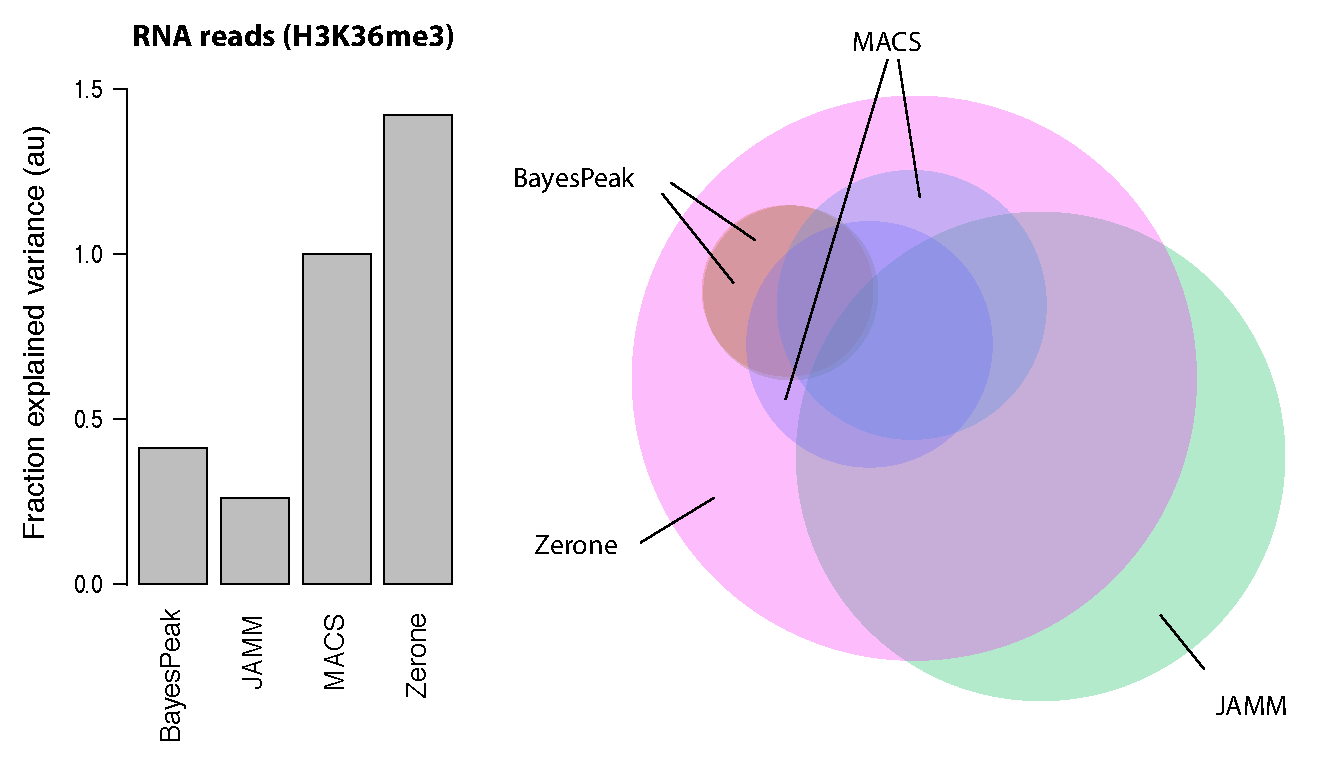
\includegraphics[scale=0.4]{histone_venn_color_names.pdf}}
\caption{
  Left panel: quality of the H3K36me3 discretization. Each bar
  represents the relative fraction of variance in RNA reads
  explained by the discretization of H3K36me3. The value for MACS was
  set to 1.0 and all other values were scaled accordingly. Right
  panel: Overlap between H3K36me3 targets (color version of the figure
  available online). Each circle represents the
  H3K36me3 targets identified by a program. The size of the circles
  is proportional to the coverage of the targets, and their overlap
  approximates the amount of targets shared by the programs. Note
  that the discretizations made by BayesPeak overlap completely and
  are indistinguishable in this representation.
}\label{fig:venn}
\end{figure}

\subsection{Speed and memory footprint}
We compared the running times of the different programs on discretizing
four data sets of similar size that represent three major types of
ChIP-seq signal. The CTCF signal consists of sharp
peaks at the transcription factor binding site, the H3K36me3 signal
consists of broad domains, and both the H3K4me3 and Pol2 signals consist
of peaks at promoters---Pol2 potentially showing broad domains on the
body of transcribed genes as well.

The results were similar between experiments for files with 7 to
36 million reads (see Table~\ref{tab:summary}). Zerone was
consistently the fastest tool, with a running time of around 5 minutes
(Fig.~\ref{fig:perf}, top row). The advantage is marginal over
MACS, which ran for around 10 minutes, but it is substantial over
JAMM and BayesPeak which ran in hours or in days, respectively.
The results for peak memory usage were variable between experiments
(Fig.~\ref{fig:perf},
bottom row). MACS achieved the best performance with a memory
footprint around 0.5~GB, followed by Zerone around 0.7~GB.
BayesPeak and JAMM each used more than 1.5~GB.

The benchmark is partly confounded by the fact that BayesPeak and MACS
discretize a single input per run, whereas Zerone and JAMM discretize
multiple inputs simultaneously. This makes a difference for pipelines
where all files have to be processed in parallel with the minimum
amount of resources. In this benchmark, Zerone processed twice as
many files per run as MACS. Per processed file, Zerone is thus
four time faster than MACS while using 30\% less memory.

\begin{figure}[!tpb]
\centerline{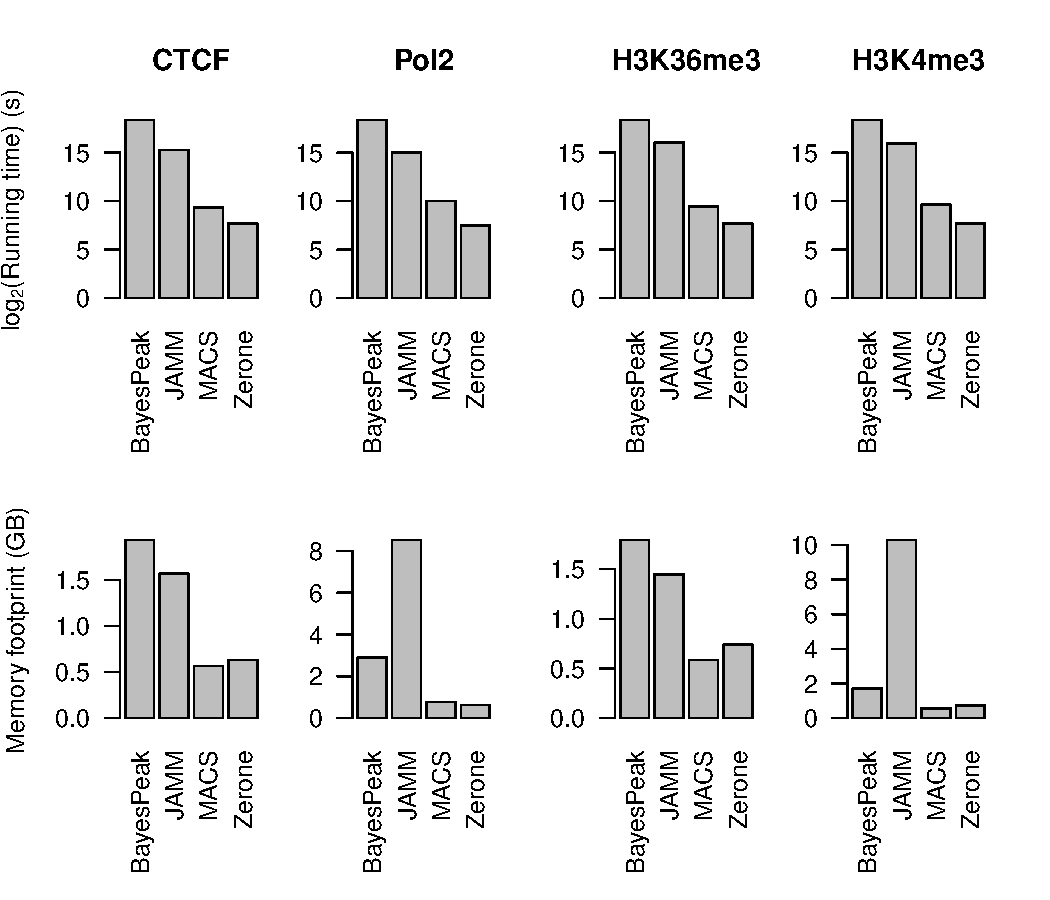
\includegraphics[scale=0.5]{performance.pdf}}
\caption{
  Running times and peak memory footprint of the
  discretizers on the four ChIP-seq data sets. For programs that only
  allow single-profile discretization (\textit{i.e.} BayesPeak and MACS),
  mean values (not the sum) are shown. The bars in dark grey represent
  the total running time when IDR is also computed (for JAMM and MACS).
  Note that the logarithmic scale misrepresents the relative fraction
  of time spent on each task.
}\label{fig:perf}
\end{figure}

\section{Discussion and conclusions}
Zerone was developed ground up for scalibility and throughput.
The result is a tool with competitive performance (Fig.~\ref{fig:perf}).
Part of the speed is due to hashing methods that dramatically
cut down the computation time during the Baum-Welch cycles. Zerone
also rests on sound statistical bases. Theoretical arguments and
experimental observations suggest that the Zero-Inflated Negative
Multinomial distribution is appropriate to model ChIP-seq data
(Fig.~\ref{fig:ZINB_fit}). This gives Zerone good specificity
and sensitivity for very different profiles (Fig.~\ref{fig:pareto}).

Zerone also proposes an original solution to the problem of
data heterogeneity. Firstly, the statistical model is fitted
in order to harmonize the replicates and solve conflicts by maximum
likelihood. Secondly, automatic quality control is performed
after the discretization. The principle of this step is somewhat
similar to anomaly detection. Note that control profiles play a key
role in the process. In order to evaluate the quality of the
discretization, Zerone implicitly assumes that the user
has provided controls that properly capture systematic biases
such as batch effects, mappability and copy number variations.

The quality control (QC) implemented in Zerone goes beyond the
Irreproducible Discovery Rate \citep[IDR,][]{li2011} in several
ways. Zerone measures the quality of the discretization and not only
the consistency between replicates. Also, the QC of Zerone is neither
limited to a specific type of profile (\textit{e.g.} sharp peaks),
nor to a preset number of replicates. Finally, issuing an
`all-or-none' call about the discretization is better practice
than silently ignoring the regions that differ between experiments
(see \textit{e.g.} Fig.~\ref{fig:jarid}).

Here we introduced a way to compare discretizers with an intuitive
graphical representation (Fig.~\ref{fig:expl}). On this plane,
the coordinates of a discretization indicate the number of targets
(or occupancy) and the amount of reads captured by these targets.
The Pareto front captures the inherent trade-off between sensitivity
and specificity in the problem of discretizing ChIP-seq profiles.
Points on this line that are close to the bottom-left corner represent
discretizations with high amount of reads per target (most specific)
and points that are close to the top-right corner represent
discretizations with many targets (most sensitive). The Pareto front
also highlights an unachievable region whose shape depends on the
structure of the signal, \textit{i.e.} on the feature being discretized
(Fig.~\ref{fig:expl}). One of the challenges of discretizing ChIP-seq
profiles is to find algorithms that perform well in all the cases.

In practice, the specificity of a discretizer is unknown because
the biological truth remains hidden. However, we can decide whether
a discretizer is more or less conservative than another by measuring
the amount of reads per target. This characteristic may be a matter of
choice, and is usually tacit in the case of ChIP-seq discretizers.
Out of two equally conservative discretizers, one may be more sensitive,
\textit{i.e.} discover more targets. The merit of the representation
introduced here is to highlight these characteristics and to guide users
when choosing the most appropriate tool for their need. Note, however,
that the number of reads per window is not the only criterion for
calling targets, so there are cases where a discretization lying
far from the front may be preferable to one lying closer to it.

This representation naturally suggests a naive approach to discretize
ChIP-seq profiles. Indeed, one could sort the genomic windows by
decreasing amount of ChIP-seq reads and declare `target' any window
above a chosen threshold. While this method would only produce
discretizations on the Pareto front, adjusting the threshold to the
conditions would be challenging for lack of an underlying model.
This is one of the major strengths of Zerone: the statistical model
automatically adjusts conservativity and sensitivity in a sensible way.

In summary, the superior performance of Zerone on different classes
of profiles, combined with the automatic quality control meet the
needs for general and robust ChIP-seq tools.

\section*{Acknowledgement}
\paragraph{Funding\textcolon}
% These acknowledgements are compliant (October 17, 2015).
The fellowship of P.C. is partly financed by the Spanish Ministry
of Economy and Competitiveness (State Training Subprogram: predoctoral
fellowships for the training of PhD students (FPI) 2013).
We acknowledge support of the Spanish Ministry of Economy and
Competitiveness, `Centro de Excelencia Severo Ochoa 2013-2017',
SEV-2012-0208. We would like to thank the anonymous reviewers
for their suggestions and their constructive criticism of the
manuscript.

\bibliographystyle{natbib}
\bibliography{document,extra}

\end{document}
